\documentclass[crop=false, class=book]{standalone}

%impostazioni lingua
\usepackage[T1]{fontenc}
\usepackage[utf8]{inputenc}
\usepackage[english,italian]{babel}

\usepackage[dvipsnames]{xcolor}
\usepackage{listings}

\lstdefinelanguage{Kotlin}{
	comment=[l]{//},
	commentstyle={\color{gray}\ttfamily},
	emph={[1]first, firstOrNull, forEach, lazy, map, mapNotNull, println},
	emphstyle={[1]\color{OrangeRed}},
	identifierstyle=\color{black},
	keywords={!in, !is, abstract, actual, annotation, as, as?, break, by, catch, class, companion, const, constructor, continue, crossinline, data, delegate, do, dynamic, else, enum, expect, external, false, field, file, final, finally, for, fun, get, if, import, in, infix, init, inline, inner, interface, internal, is, lateinit, noinline, null, object, open, operator, out, override, package, param, private, property, protected, public, receiveris, reified, return, return@, sealed, set, setparam, super, suspend, tailrec, this, throw, true, try, typealias, typeof, val, var, vararg, when, where, while, it},
	keywordstyle={\color{NavyBlue}\bfseries},
	morecomment=[s]{/*}{*/},
	morestring=[b]",
	morestring=[s]{"""*}{*"""},
	ndkeywords={@Deprecated, @JvmField, @JvmName, @JvmOverloads, @JvmStatic, @JvmSynthetic, Array, Byte, Double, Float, Int, Integer, Iterable, Long, Runnable, Short, String, Any, Unit, Nothing, Config, LightEstimationMode, CameraConfigFilter, CameraConfig, FacingDirection, AugmentedFaceMode, AugmentedFace, TrackingState, RegionType, CloudAnchorMode,AugmentedImageDatabase, BitmapFactory, Session, InstantPlacementMode, File, Uri, RecordingConfig },
	ndkeywordstyle={\color{BurntOrange}\bfseries},
	sensitive=true,
	stringstyle={\color{ForestGreen}\ttfamily},
	emph={[2]FRONT,MESH3D,ENVIRONMENTAL\_HDR,AMBIENT\_INTENSITY, DISABLED,FOREHEAD\_LEFT,FOREHEAD\_RIGHT,NOSE\_TIP, TRACKING, ENABLED, LOCAL\_Y\_UP},
	emphstyle={[2]\color{Purple}\ttfamily},
}

\definecolor{lightgrey}{RGB}{230,237,244}

\lstset{
	basicstyle=\scriptsize\sffamily\color{black},
	backgroundcolor=\color{lightgrey},
	frame=single,
	numbers=left,
	numbersep=5pt,
	numberstyle=\tiny\color{gray},
	showspaces=false,
	showstringspaces=false,
	tabsize=1,
	texcl=true,
	captionpos=b,
	breaklines=true
}




%sistema i margini
\usepackage{geometry}
\geometry{a4paper,top=2.2cm,bottom=2.2cm,left=3cm,right=3cm, heightrounded}

%interlinea 1.5
\usepackage{setspace}
\onehalfspacing

%gestione delle testatine
\usepackage{fancyhdr}
\pagestyle{fancy}
\lhead{}
\chead{}
\rhead{Titolo}
\lfoot{}
\cfoot{\thepage}
\rfoot{}
\renewcommand{\headrulewidth}{0.4pt}

%formattazione titoli paragrafo
\usepackage{titlesec}
\titleformat{\chapter}[block]{\normalfont\huge\bfseries}{\thechapter.}{0.7em}{\huge}

%pacchetti per i riferimenti in bibliografia
\usepackage[autostyle,italian=guillemets]{csquotes}
\usepackage[style=numeric,citestyle=numeric-comp,backend=biber]{biblatex}

%risorsa che contiene la bibliografia
\addbibresource{./../bibliografia.bib}

\usepackage{lipsum}
\usepackage{graphicx}
\usepackage[italian]{varioref}
\usepackage{copyrightbox}
\usepackage{subfig}

\begin{document}
		
	\chapter{Anchor and Trackable}
	
		ARCore definisce gli Anchor per assicurare che gli oggetti virtuali rimangano nella stessa posizione e vengano 					tracciati nel tempo. L'ambiente circostante può cambiare, ed è necessario che la posizione di questi oggetti
		rimanga stabile. Gli Anchor sono disposti in insieme di punti o piani rappresentati da oggetti di tipo Trackable.\\
		Gli oggetti Trackable rappresentano la forma geometrica sulla quale verranno definiti gli anchor.
		Su questi oggetti possono essere invocati 3 metodi:
		\begin{itemize}
			\item[•] \emph{createAnchor(pose: Pose)} crea un anchor in una posa che è definita nel Trackable corrente. Il tipo di oggetto Trackable definirà il modo con cui l'anchor verrà disposto e la modalità di aggiornamento della sua posa mentre il modello del mondo varia.
			\item[•] \emph{ getAnchors()} restituisce tutti gli anchor presenti nel dato Trackable.
			\item[•] \emph{getTrackingState()} restituisce un oggetto TrackingState che rappresenta lo stato del Trackable. Questo stato può essere: PAUSED quando il rilevamento viene perso ma potrebbe riprendere in futuro; STOPPED quando viene fermato e non verrà più ripreso; TRACKING se viene tracciato il determinato Trackable.
		\end{itemize}
		\begin{flushleft}
			La definizione di anchor e lo stato di tracciamento sono stati molto importanti per la definizione delle 						funzionalità principali della nostra applicazione.\\
	 		In base alla modalità l'applicazione offre funzionalità differenti:
		\end{flushleft}
	 	\begin{itemize}
	 		\item \emph{Plane Detection}: ARCore rileva dei piani (Trackable) sui quali è possibile posizionare degli animali virtuali. In particolare, quando l'utente tocca un punto preciso del piano viene definito un anchor sul quale verrà renderizzato il modello 3d dell'animale. (Codice in \vref{lst: Definizione Anchor in Plane Detection})
	 	
	 		\item \emph{Augmented Images}: in ciascun frame viene controllato se lo stato di un'immagine aumentata è TRACKING; in questo caso l'immagine viene riconosciuta e viene definito un anchor nel suo centro nel quale verrà renderizzato il modello del pianeta corrispondente. (Codice in \vref{lst: Definizione Anchor in Augmented Images})
	 	\end{itemize}
		
		\clearpage
		\begin{center}
				\begin{minipage}{1.1\textwidth}
					\begin{lstlisting}[caption={Definizione Anchor in Plane Detection}, label={lst: Definizione Anchor in Plane Detection}, language=Kotlin]
					 //Evento che si verifica quando viene toccato un piano
            		 arFragment.setOnTapArPlaneListener { hitResult, plane, motionEvent ->

                	 //Se siamo nella modalità place model
                	 if (!switchButton.isChecked) {

                     arFragment.arSceneView.scene.addChild(AnchorNode(hitResult.createAnchor()).apply {
 
                        // Crea il transformable model e lo aggiunge all'anchor
                        addChild(TransformableNode(arFragment.transformationSystem).apply {

                            setModel()
                            renderable = objRenderable
                            
                            //...
					
						\end{lstlisting}
					\end{minipage}
				\end{center}
			\vspace{0.2cm}
		\begin{center}
			\begin{minipage}{1.1\textwidth}
				\begin{lstlisting}[caption={Definizione Anchor in Augmented Images}, label={lst: Definizione Anchor in Augmented Images}, 	language=Kotlin]
				//Per ogni immagine tracciata  se non è presente il  modello allora viene immediatamente costruito e instanziato
        		for (augmentedImage in augmentedImages) {

            		if (augmentedImage.trackingState == TrackingState.TRACKING) {

                		for (i in 0 until namesobj.size) {

                    		if (augmentedImage.name.contains(namesobj[i]) && !renderobj[i]) {

                        		Toast.makeText(this,""+namesobj[i]+" rilevato",Toast.LENGTH_SHORT).show()

                        		if(namesobj[i]=="systemsolar"){
                            		renderObject(
                                		arFragment,
                                		augmentedImage.createAnchor(augmentedImage.centerPose),
                                		"solar_system"
                            		)
                        		}else {
                            		renderObject(
                                		arFragment,
                                		augmentedImage.createAnchor(augmentedImage.centerPose),
                                		namesobj[i]
                            		)
                        		}	
                        		renderobj[i] = true
                    		}
                		}
            		}
        		}
					\end{lstlisting}
			\end{minipage}
		\end{center}
	
		\clearpage
		
		\begin{flushleft}
			Di seguito è riportata una rappresentazione di come un oggetto virtuale viene disposto in un piano.
		\end{flushleft}
		\begin{figure}
				\centering
				\copyrightbox[0.5]{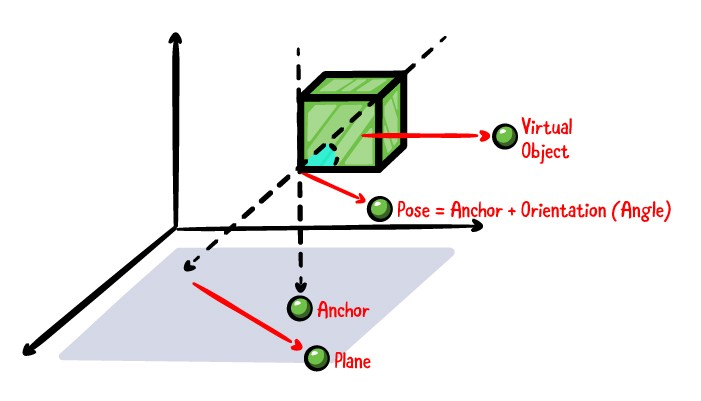
\includegraphics[width=0.7\textwidth]{../../resources/images/UserInteraction/Anchor.jpeg}}%
				{Fonte: \url{https://medium.com/@jaaveeth.developer/arcore-81528569eb2c}}
				\caption{Oggetto virtuale in un piano}
				\label{fig: Oggetto virtuale in un piano}
		\end{figure}	

	\begin{flushleft}
		Nella modalità \emph{Plane Detection} la posa (posizione e orientamento) di un animale rimane invariata anche se 				l'ambiente circostante cambia.\\
		Qui sotto sono riportati degli esempi in cui si può notare che il pinguino rimane nello stesso punto da qualsiasi 				prospettiva e distanza.
	\end{flushleft}
	
	\begin{figure}
			\centering
			\copyrightbox[b]{
				\subfloat[][\emph{Pinguino da un'inquadratura vicina}]
				{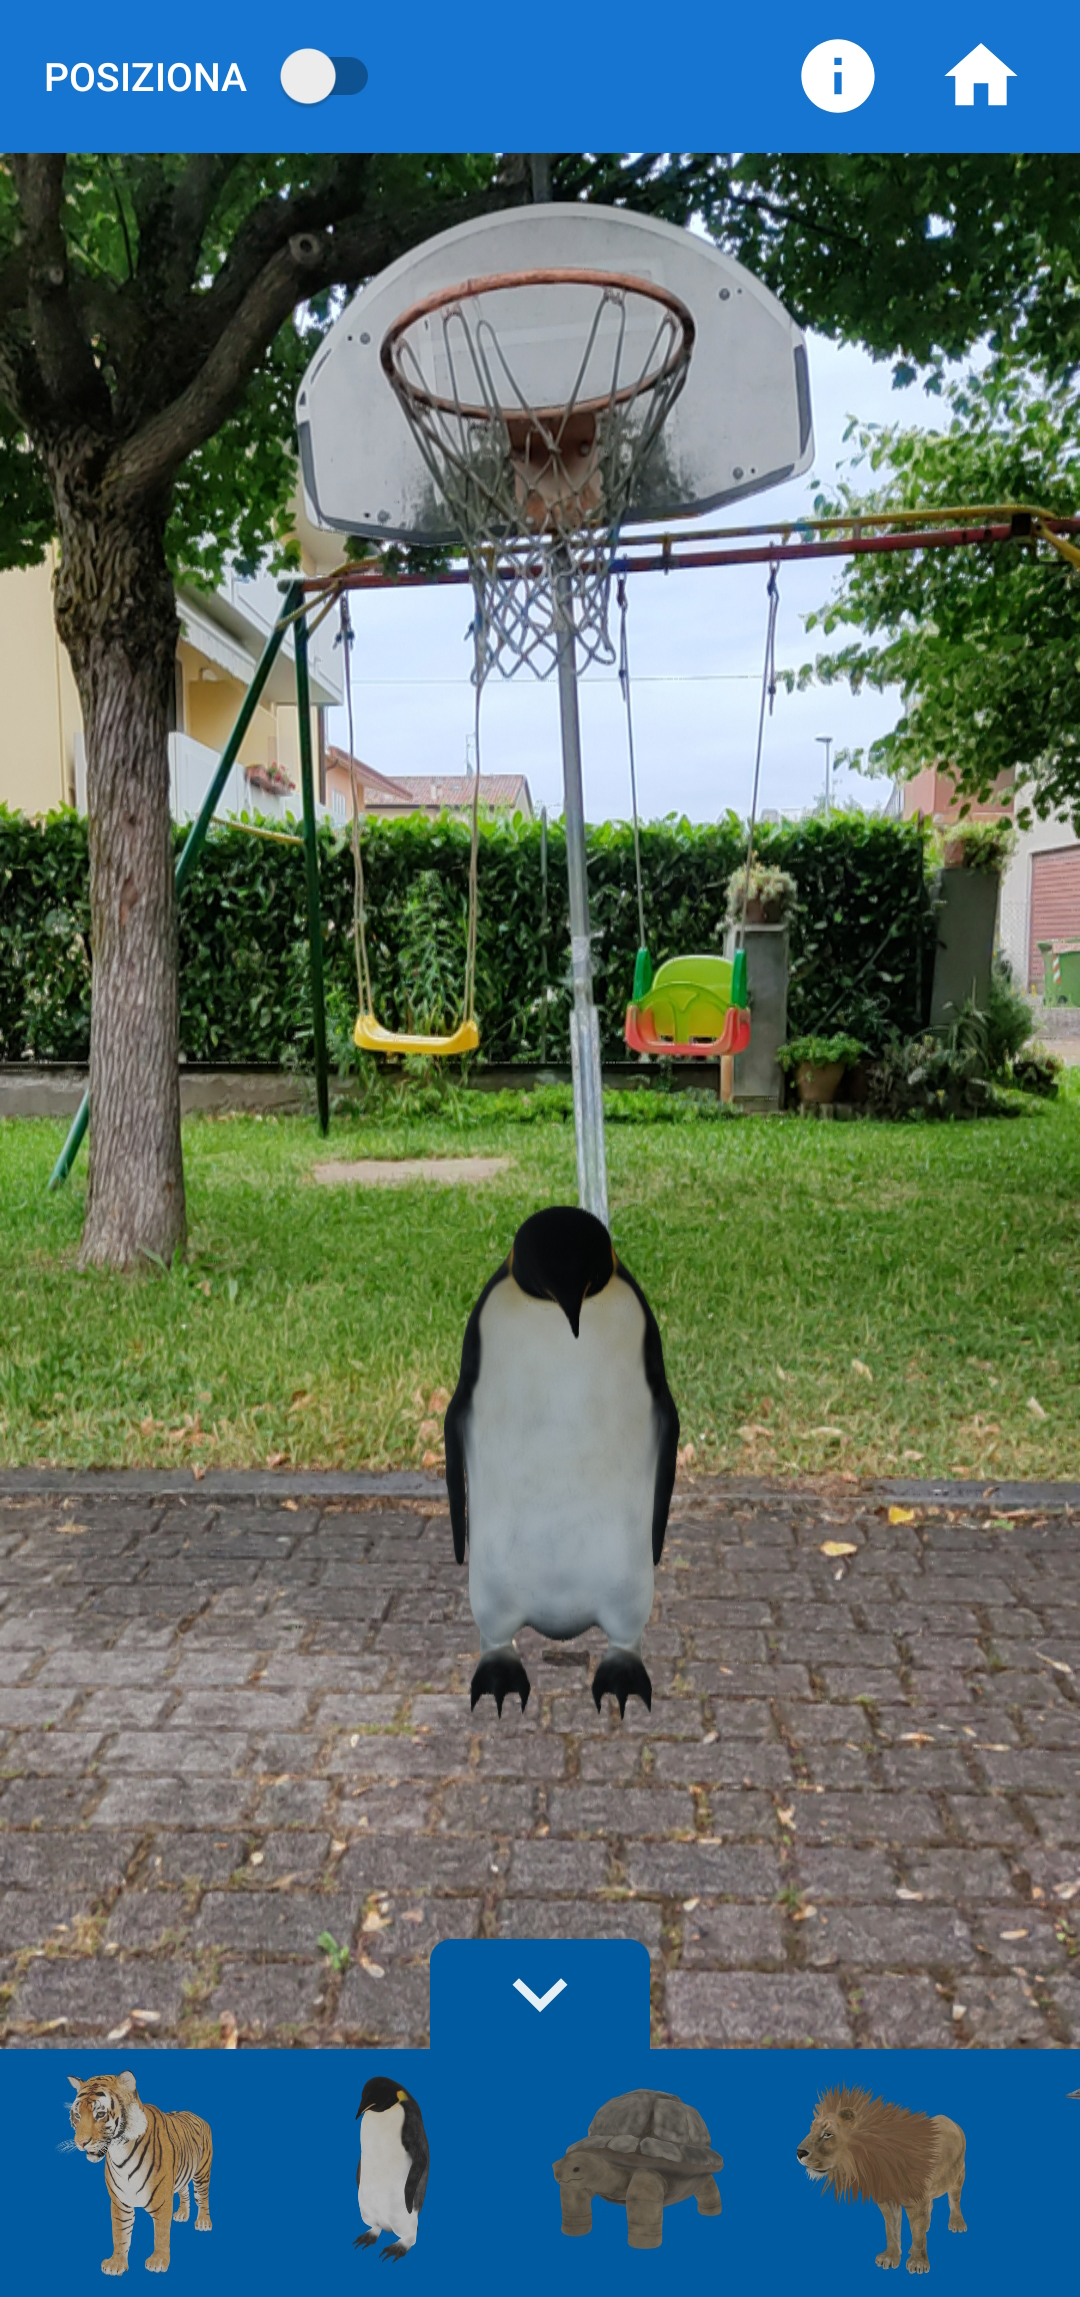
\includegraphics[width=0.28\textwidth]{../../resources/images/AnchorTrackable/pingvicino.jpg}}  \quad,
				\subfloat[][\emph{Pinguino da un'inquadratura lontana}]
				{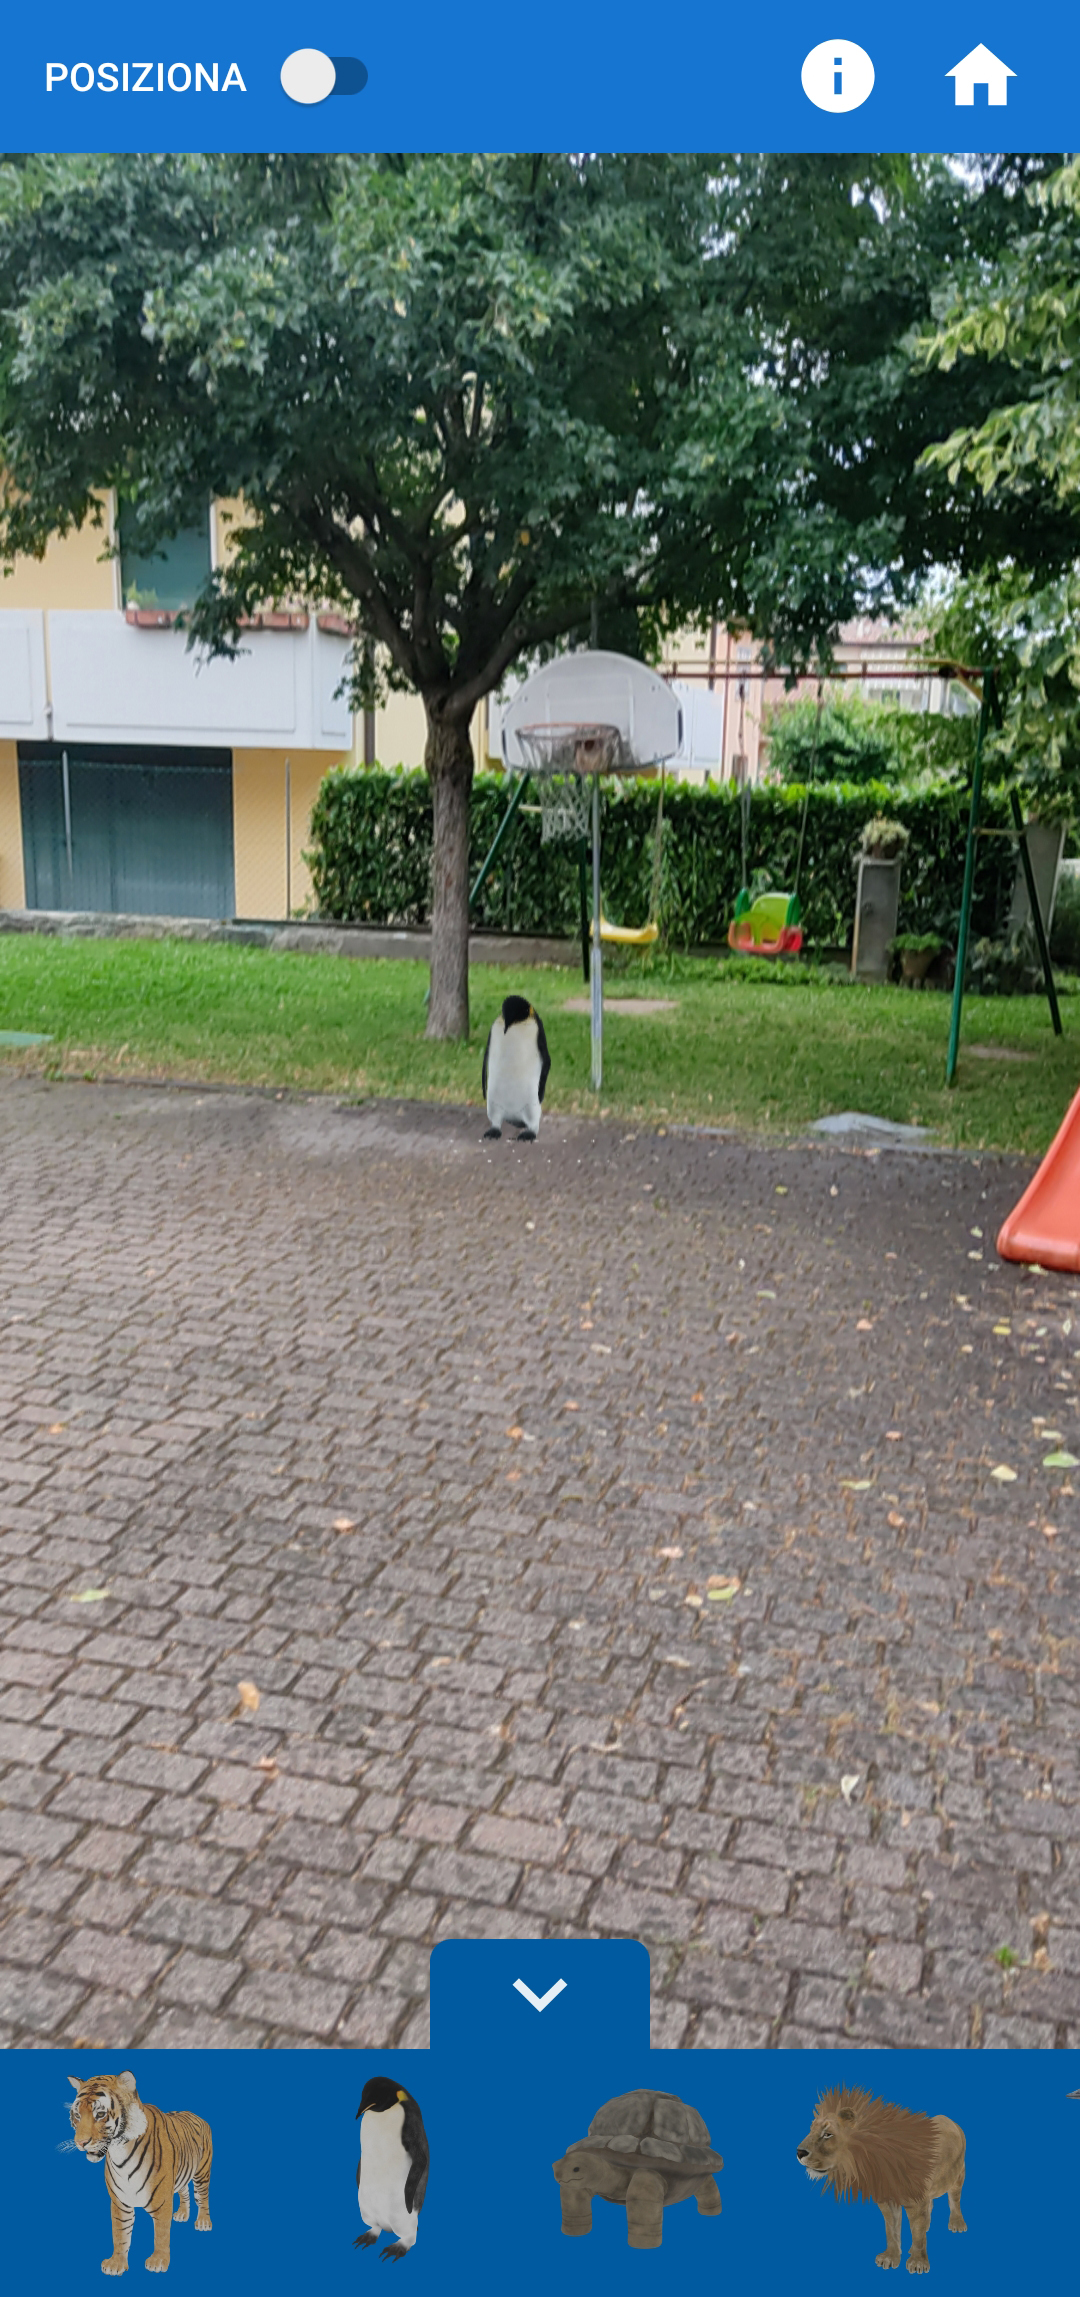
\includegraphics[width=0.28\textwidth]{../../resources/images/AnchorTrackable/pinglontano1.jpg}} \quad,
				\subfloat[][\emph{Giove da lontano}]
				{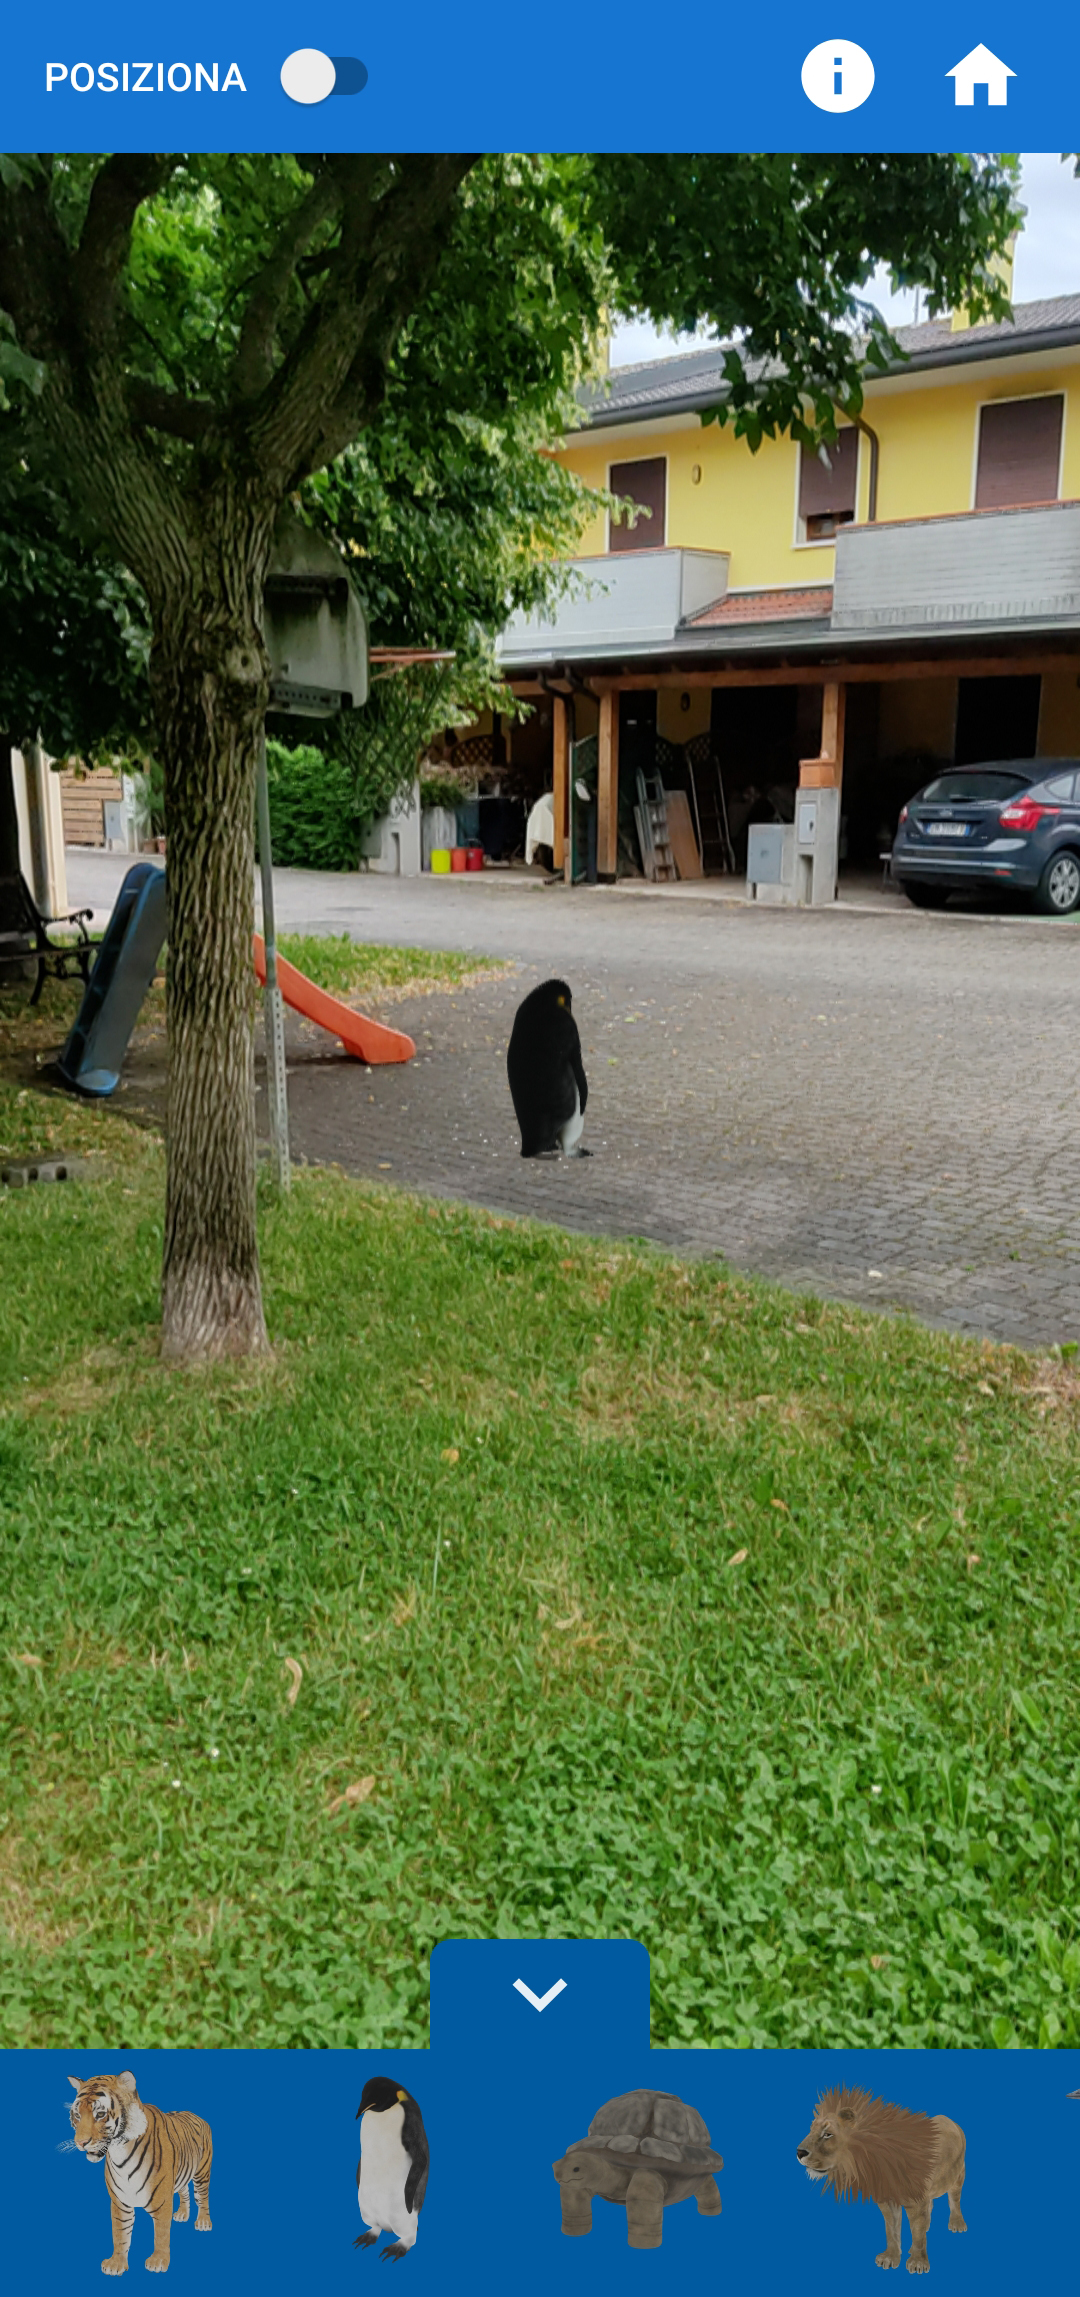
\includegraphics[width=0.28\textwidth]{../../resources/images/AnchorTrackable/pinglontano2.jpg}}
			}{Fonte: \url{https://developers.google.com/}}	
			\caption{Esempio di inquadrature differenti in Plane Detection}
			\label{fig:augm_img}
		\end{figure}	
	
		
	\begin{figure}
			\centering
			\copyrightbox[b]{
				\subfloat[][\emph{Tracciamento immagine}]
				{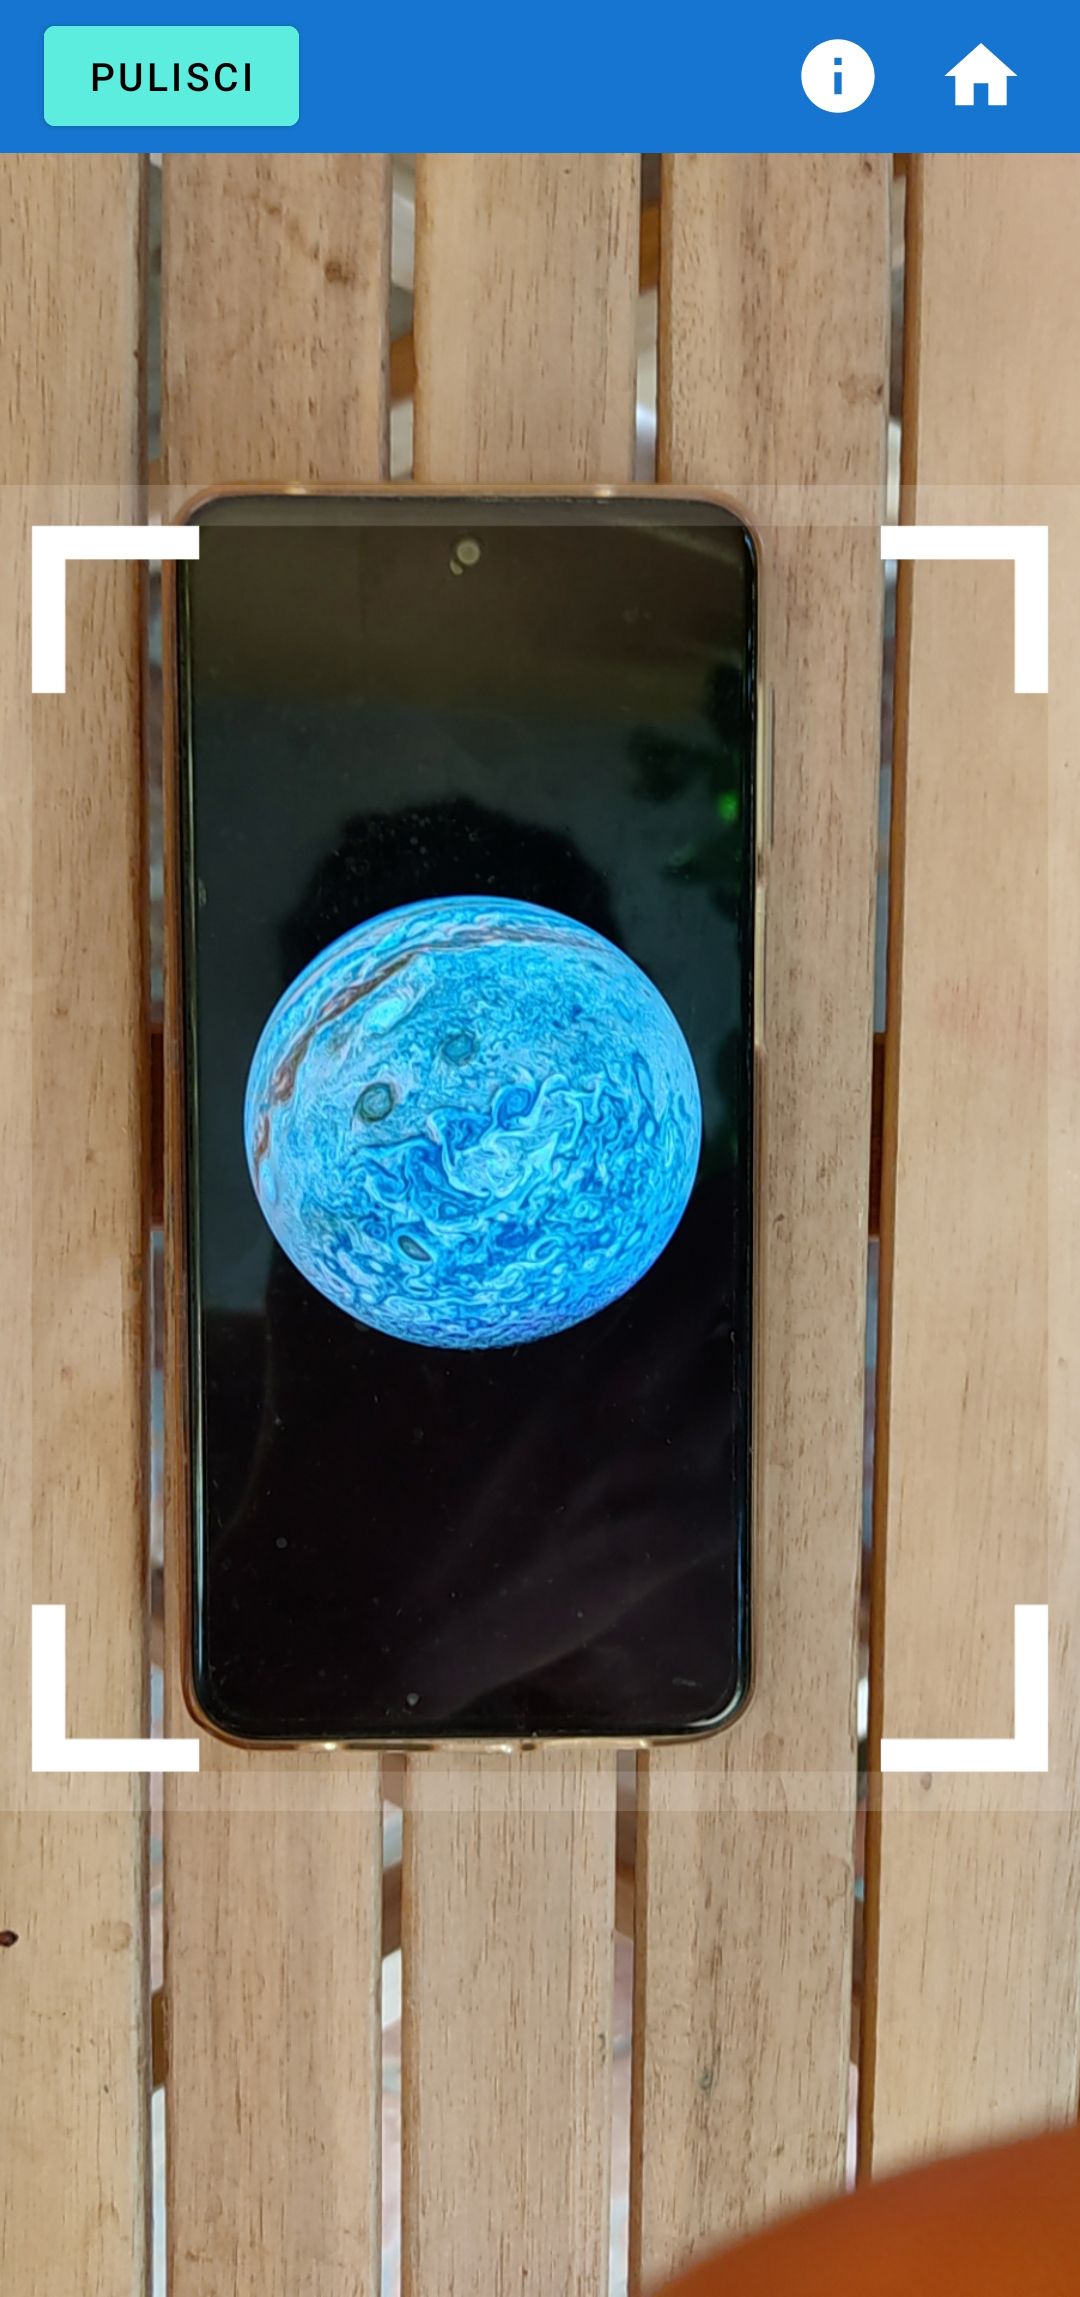
\includegraphics[width=0.28\textwidth]{../../resources/images/AnchorTrackable/Giove2d.jpg}}  \,
				\subfloat[][\emph{Giove da vicino}]
				{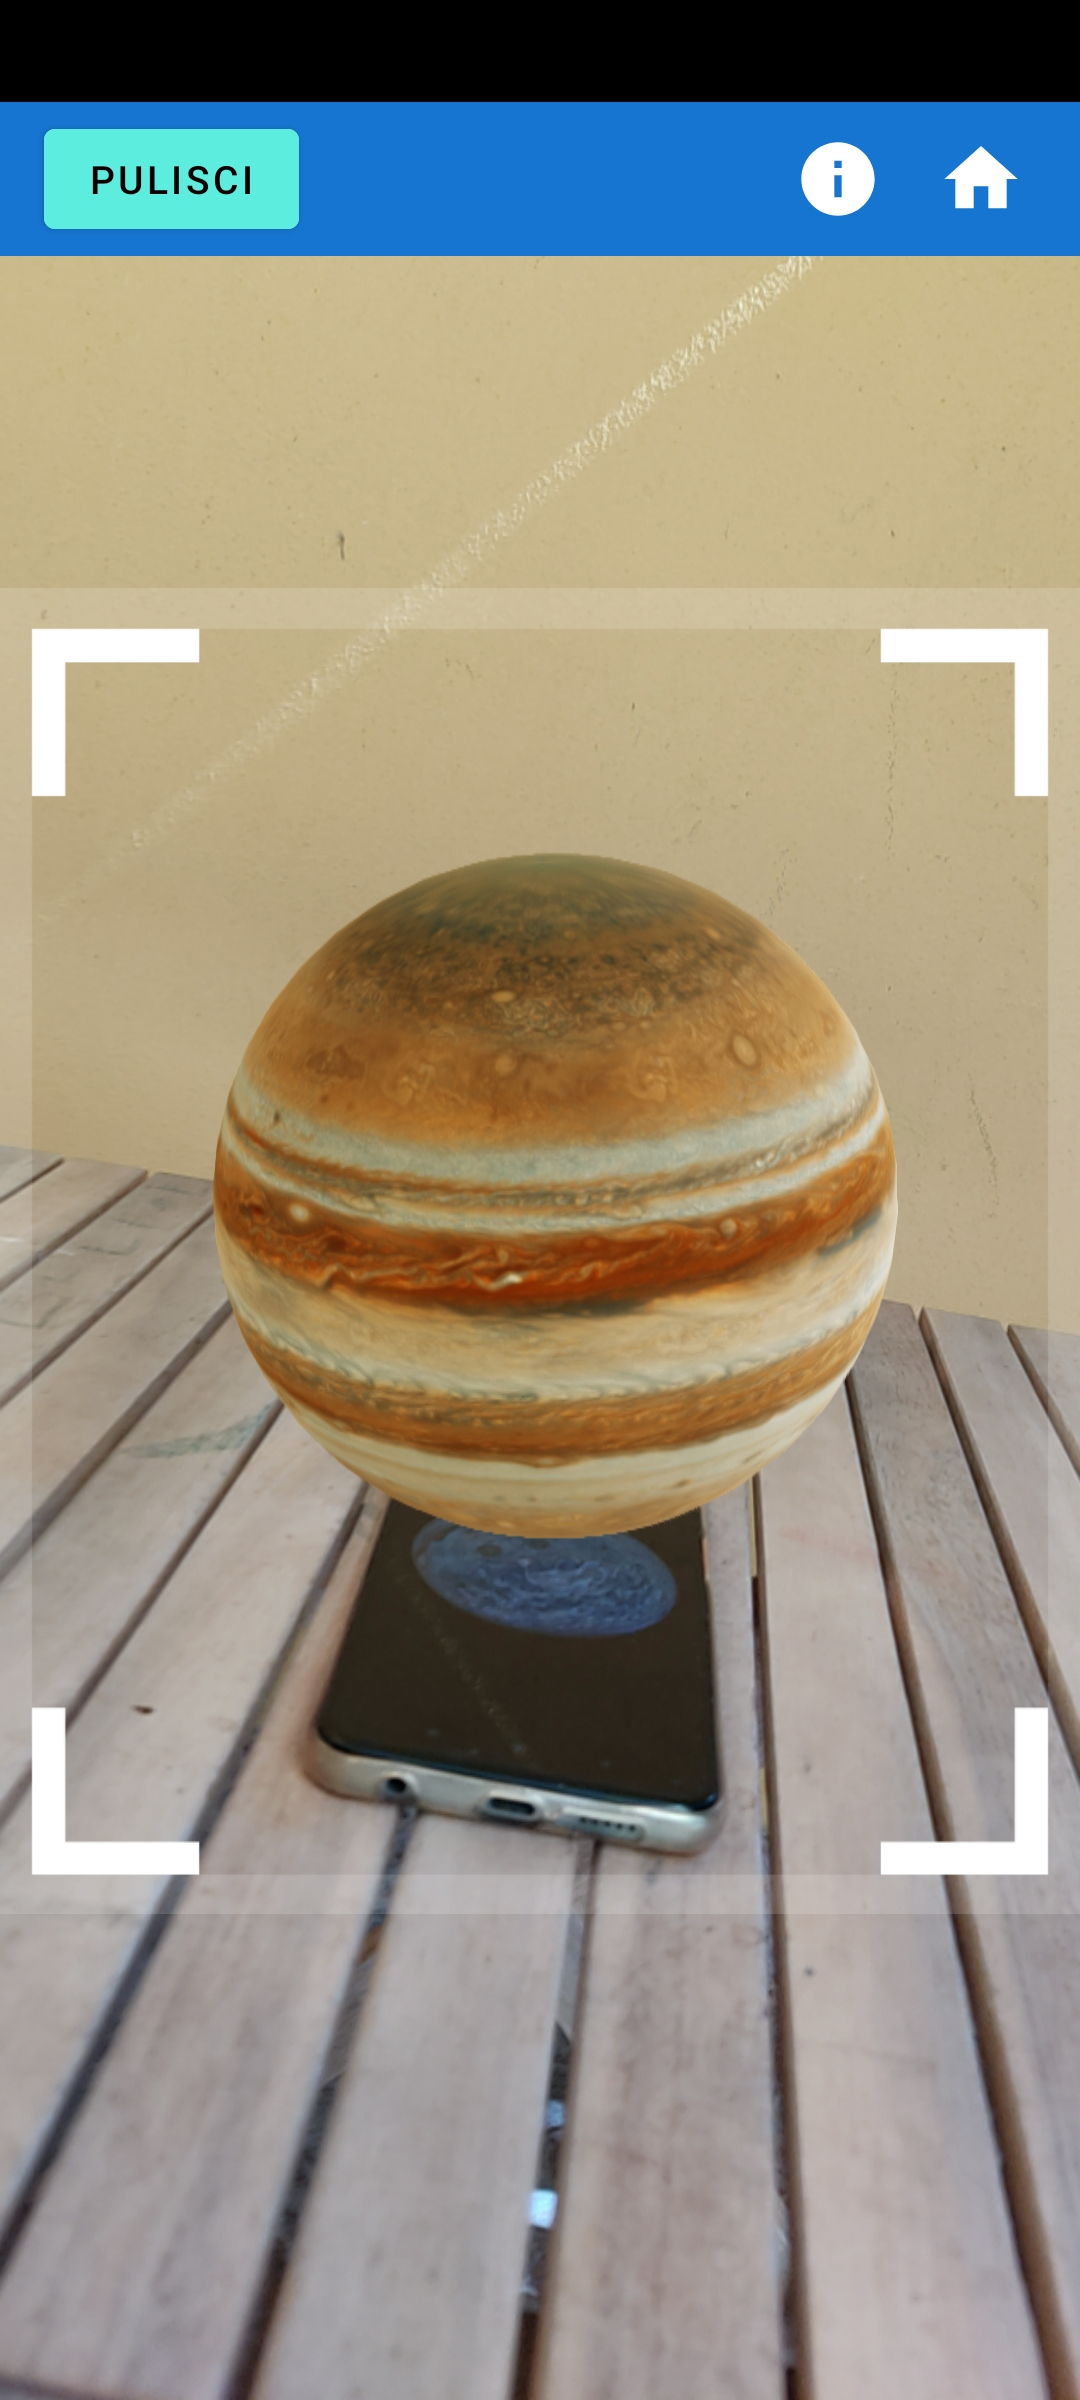
\includegraphics[width=0.28\textwidth]{../../resources/images/AnchorTrackable/GioveVicino.jpg}} \,
				\subfloat[][\emph{Giove da lontano}]
				{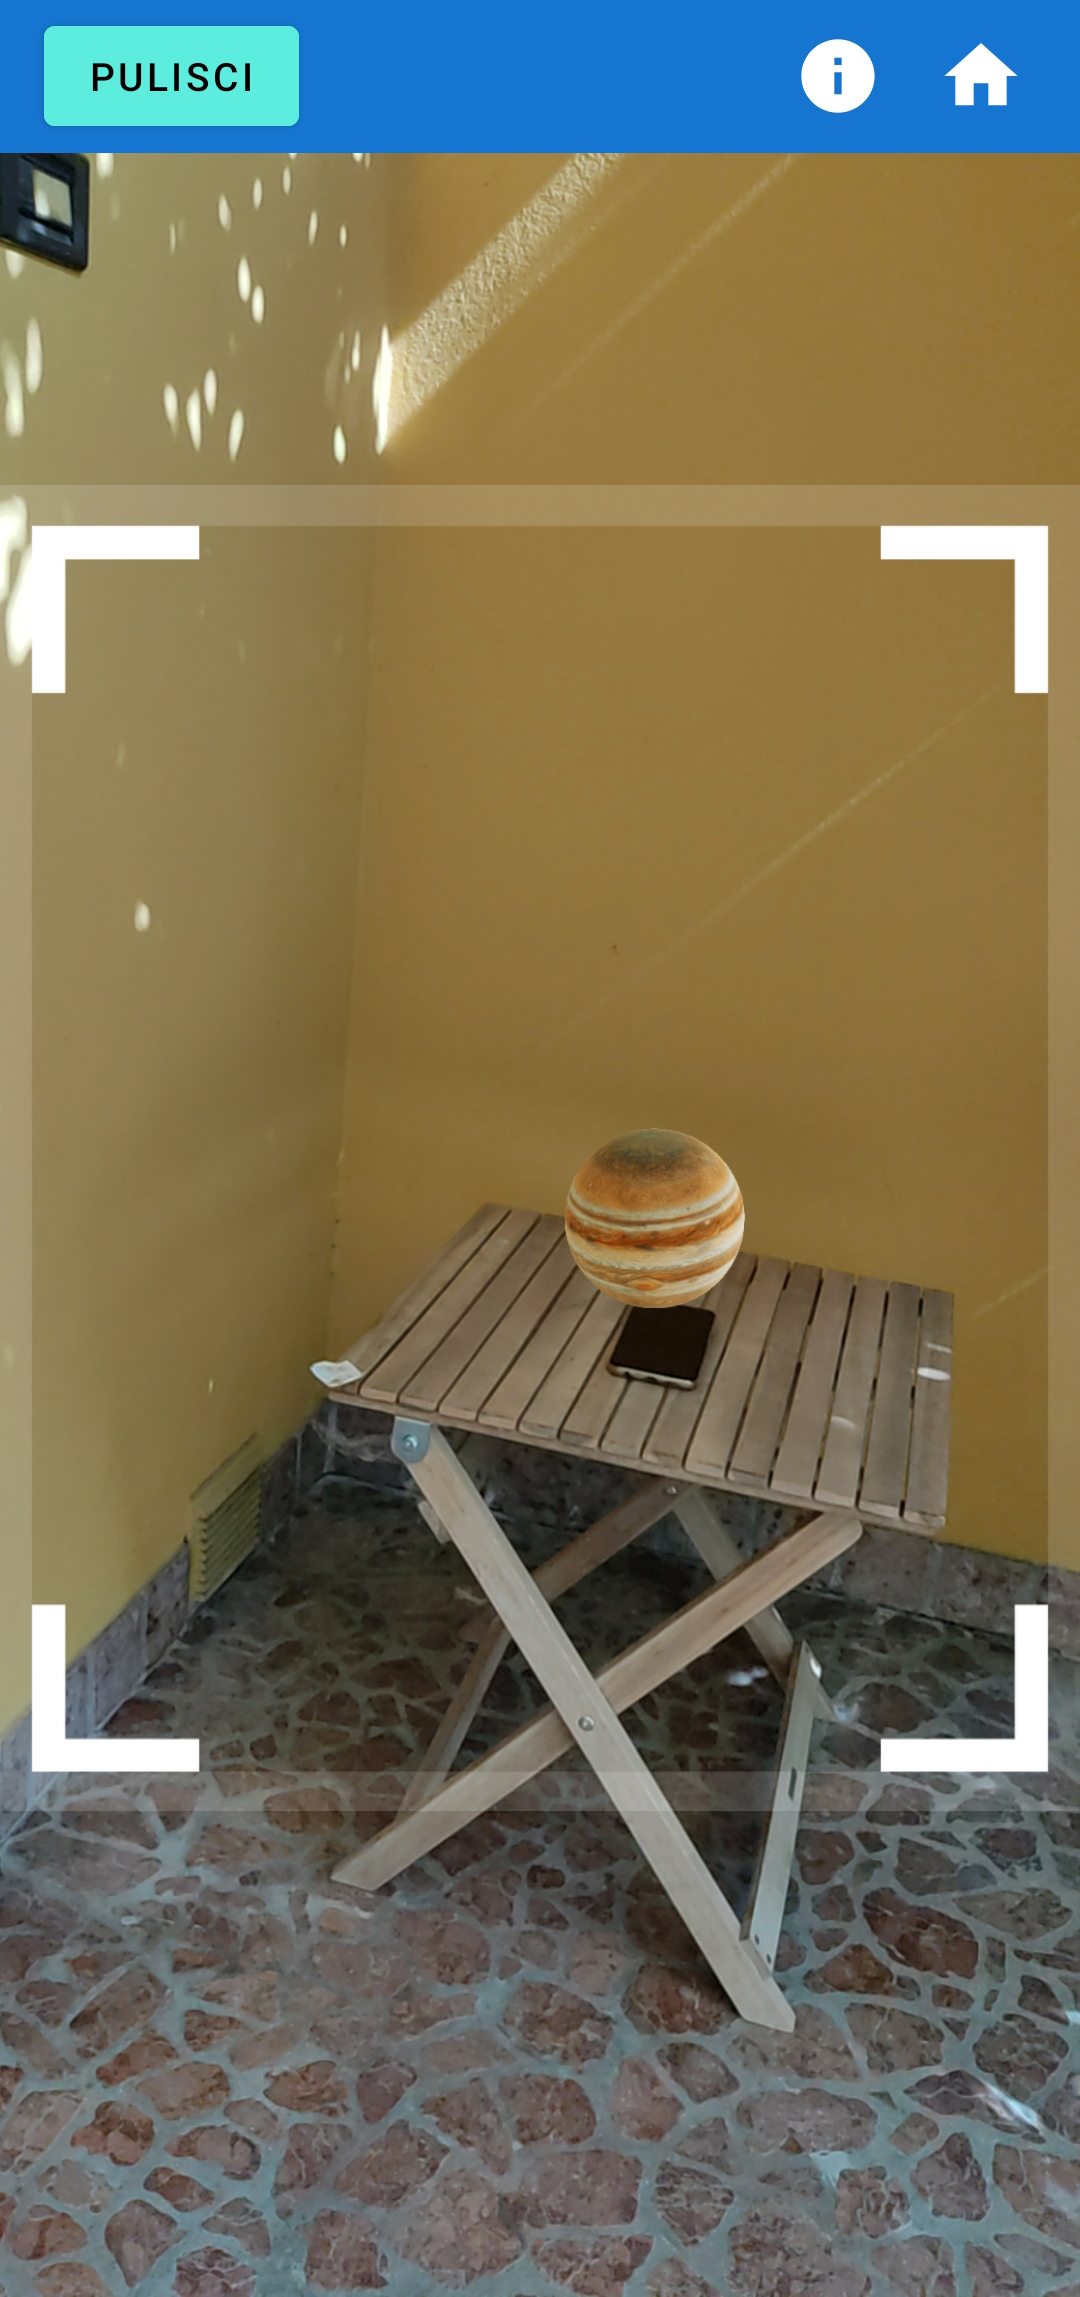
\includegraphics[width=0.28\textwidth]{../../resources/images/AnchorTrackable/GioveLontano.jpg}}
			}{Fonte: \url{https://developers.google.com/}}	
			\caption{Esempio di rilevamento in Augmented Images}
			\label{fig:augm_img}
		\end{figure}
\end{document}